\documentclass[assd_tp3_main.tex]{subfiles}

\begin{document}

\section{Conversores $\Sigma\Delta$}
Los conversores $\Sigma\Delta$ destacan por brindar la posibilidad de tener un buen rango dinámico siempre que
la señal a digitalizar no se extienda en un amplio rango de frecuencia.
Para poder desarrollar los temas se requiere un conocimiento previo de teorema del muestreo y muestreo pasabanda.
\subsection{Error de cuantización}
La cuantización es convertir una muestra de valor continuo x a un conjunto finito de valores discretos $q_i$.
M es la cantidad de valores $q_i$ que esta determinada por el tipo de cuantizador  su funcion transferencia q(x).
Para un cuantizador uniforme, los subintervalos $\Delta=q_{i+1}-q_i$ son iguales. Este tipo de cuantizador es más común pero no siempre es el más eficiente.
La diferencia $e(n)=q_i(n)-x(n)$ se llama error de cuantización. El mismo está en el orden de $\Delta$.
Cabe aclarar que si se va de escala la señal introducida $\Delta$ toma un valor mayor que el establecido.
Como la señal digital final es representada en un valor binario de B bits entonces hay un total de $M=2^{B}$ niveles de cuantización disponibles.
Asumiendo que la secuencia x(n) es escalada de forma tal que $|x(n)|\leq1$ entonces como $x_{max} =1$ y $x_{min} =-1$:
\[ \Delta= \frac{2}{2^B-1} \]
El error de cuantización e(n) debido a que se obtiene por aproximar al valor mas cercano, tiene un máximo valor absoluto de $0.5\Delta$.
Se sigue que:
\[ x_q(n)= x(n)+e(n)\]
En donde e(n) se lo llamará de ahora en más ruido de cuantización.
\begin{figure}[H]
\centering
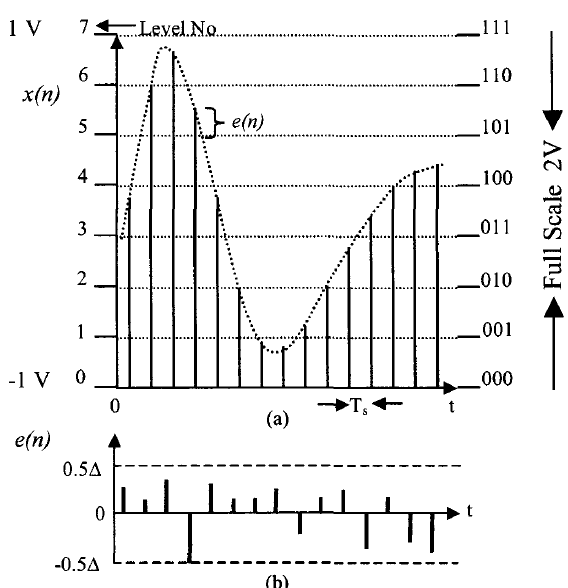
\includegraphics[width=0.52\linewidth]{images/ej4/quant_err.png}
\caption{En los procesos de cuantizacion los valores de las muestras son redondeadas al nivel más cerca disponible y luego son representadas en binario. La alteración de las muestras iniciales converge en el ruido de cuantización e(n)}
\label{fig:quant_err}
\end{figure}
El ruido de cuantización e(n) es casi incorrelacionado con la señal de entrada, tiene un espectro blanco y su distribución de probabilidad es uniforme en el rango $[-\Delta/2,\Delta/2]$
Como consecuencia el error de cuantización puede pensarse como una fuente de ruido blanco aditivo e independiente.

Se define el SQRN como la relación Señal-Ruido de cuantización:
\[ SQNR= \frac{PotSenal}{PotRuidoCuantizado}\]

\begin{figure}[H]
\centering
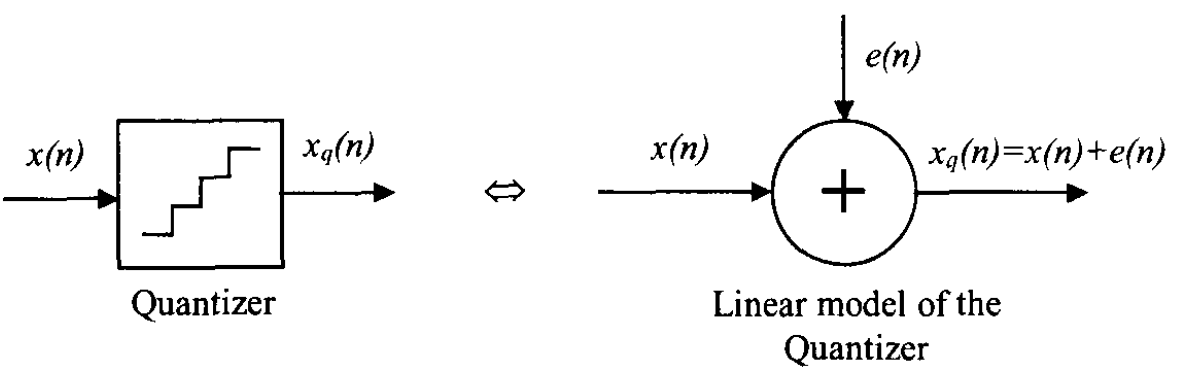
\includegraphics[width=0.52\linewidth]{images/ej4/cuantmodel.png}
\caption{Modelo lineal para el cuantizador}
\label{fig:cuantmodel}
\end{figure}


Por ser uniforme en $[-\Delta/2,\Delta/2]$:\\
\[ \mu_e = 0 \]
\[ \sigma_e^2 = \frac{\Delta^2}{12} \]
Si los valores de e(n) se asumen incorrelacionados e identicamente distribuidos el ruido de cuantización es blanco y su potencia es distribuida uniformemente sobre todo el rango de $[-f_s/2,f_s/2]$. Por tanto, la densidad espectral de potencia en el ruido N(f) puede ser expresada como:
\[ N(f)=\frac{\Delta^2}{12f_s} \]
Para una senoidad con variación de amplitud en escala completa\\ 
$2A =(2^B-1)\Delta$, su potencia es $A^2/2$ y el SQRN es:\\
\[ SQRN=10log\left( \frac{A^2/2}{\sigma_e^2} \right)\approx10log\left(\frac{3\cdot2^{2B}}{2}\right)=(6.02 \cdot B+1.76)dB \]
Se concluye que si se incrementa en uno el número de bits, se aumenta el SQNR en 6dB.
De hecho, esto nos da pie a pensar el máximo número de bits que se necesita para cuantizar una señal analógica con un piso de ruido específico.
Una característica que se debe destacar de un cuantizador es su rango dinámico. 
\[ rango\,dinamico=log_2\frac{x_{max}}{\Delta/2}\]

\todo[inline]{Aca se supone que va la foto del ruido desplazado.\newline Here's another line.}

\subsection{Principios de Oversampling}
Los requerimientos de alta resolución y rango dinámico en el procesamiento de señales no puede ser logrado con los ADCs convencionales, debido a las limitaciones de sus implementaciones.
\begin{itemize}
\item La implementación de cuantizadores uniformes con un gran número de niveles de cuantización. Para un succesive aproximation ADC con 16 bits de precisión, $2^16=65536$ niveles equidistantes deben ser determinados.
\item La implementación del FAA con requerimientos estrictos tales como una banda angosta de transición, alta atenuación en la banda de rechazo, muy poco ripple en la banda pasante ,fase lineal, bajo ruido, etc. Tales especificaciones no se pueden lograr con circuitos integrados analógicos.
\item La presencia del efecto Jitter, por ejemplo la incertidumble en el tiempo de flancos del pulso de clock usados en el muestreador. 
\end{itemize}
Una manera de mejorar esta situación es incrementar la tasa de muestreo mucho más que la de los ADCs convencionales, por ejemplo arriba de Nyquist $(f_{N}=2f_b)$. Desde luego que requiere que varios componentes del ADC operen a una frecuencia mucho más alta. Muestrear a una $f_s$ mas grande que la de Nyquist se la suele llamar $\bold{oversampling}$.
Una medida del oversampling es la llamada Oversampling Ratio (OSR) deinida como R:
\[ R=\frac{f_s}{f_N} \]
En general R es un número potencia de 2. Si el R está entre 2 y 16 hablamos de un grado leve de oversampling mientras que un fuerte oversampling ocurre cuando R está entre 16 y 256.



\subsection{Moduladores $\Sigma\Delta$ de primer orden }
Recordamos dos características importantes del modulador:
\begin{itemize}
\item \textbf{Oversampling}: distribuye el ruido de cuantización 
\item \textbf{Noise shaping}: expulsa la mayoría del ruido que estaba dentro de la banda a frecuencias altas. 
\end{itemize}
A continuación se presentan diagramas en bloques del modulador $\Sigma\Delta$ de primer orden.
\begin{figure}[H]
\centering
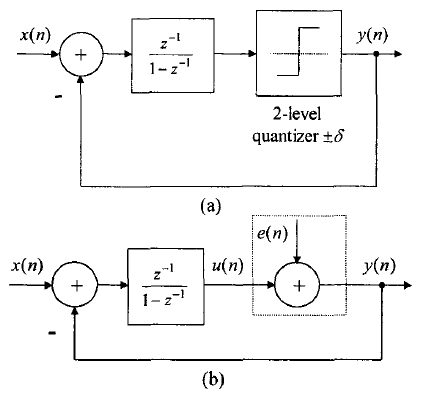
\includegraphics[width=0.4\linewidth]{images/ej4/sd_linmodel.png}
\caption{Diagrama en bloques del modulador $\Sigma\Delta$(a) y su modelo lineal(b)}
\label{fig:sigmadelmod_model}
\end{figure}
La señal e(n) en el modelo lineal de la figura \ref{fig:sigmadelmod_model} se la llama ruido de cuantización.
\[ y(n)=x_q(n)= u(n)+e(n) \]
De la figura \ref{fig:sigmadelmod_model} obtenemos la SignalTransferFunction (STF) y la NoiseTransferFunction (NTF):
\[ Y(z)= z^{-1}X(z)+(1-z^{-1})E(z) \]
\[ STF(z)= z^{-1} \]
\[ NTF(z)= 1-z^{-1} \]


\end{document}
